\chapter[Datos]{Datos}
\label{Chap2}

Navarra dispone de dos confederaciones hidrográficas, la del cantábrico y la del ebro. Estas son organismos encargados de la gestión de cuencas hidrográficas que discurren por múltiples comunidades autónomas. Tomando como cuenca hidrográfica a la superficie por la cual fluye un conjunto de agua, como ríos, arroyos y lagos hasta su desembocadura en el mar.\newline
\newline
La del cantábrico ejerce sobre aquellos ríos cuya desembocadura va a parar al cantábrico, mientras, la del ebro trabaja sobre las zonas limitadas al cauce del ebro.\newline
\newline
No se hace uso de la página de la confederación del ebro al disponer de datos de otras páginas como la de la agencia estatal de meteorología y, la de agua en navarra. 

\begin{figure} [H]
	\centering
	\includegraphics[width=0.7\textwidth]{fig/ConfederacionesHidrográficas.jpg}
	\caption[Confederaciones hidrográficas en España]{Confederaciones hidrográficas en España}
	\label{fig:ej32}
\end{figure}

Creadas en 1926, las confederaciones, mostradas en la figura \ref{fig:ej32}, son organismos autónomos, con plena autonomía funcional, adscritas al Ministerio para la Transición Ecológica y el Reto Demográfico. El papel desempeñado por estas recae entre otras cosas en, la planificación hidrológica, gestión de recursos y aprovechamientos, protección del dominio público hidráulico, control de calidad del agua y los bancos de datos.\newline
\newline
Por todo esto, es de gran importancia para este proyecto la adquisición de datos relacionados a estas entidades que ejercen en Navarra.

\section{CHCantábrico}
En la sección de nivel del río de la pagina de CHCantábrico, se encuentra la tabla con las estaciones, mostrada en la figura \ref{fig:ej30}. Una peculiaridad de esta, es que aun seguir una estructuración típica de tabla mediante el uso de \textit{table}, dispone de una tabla adicional en cada una de las filas. como se ve en el código \ref{cod:104}.

\begin{figure} [H]
	\centering
	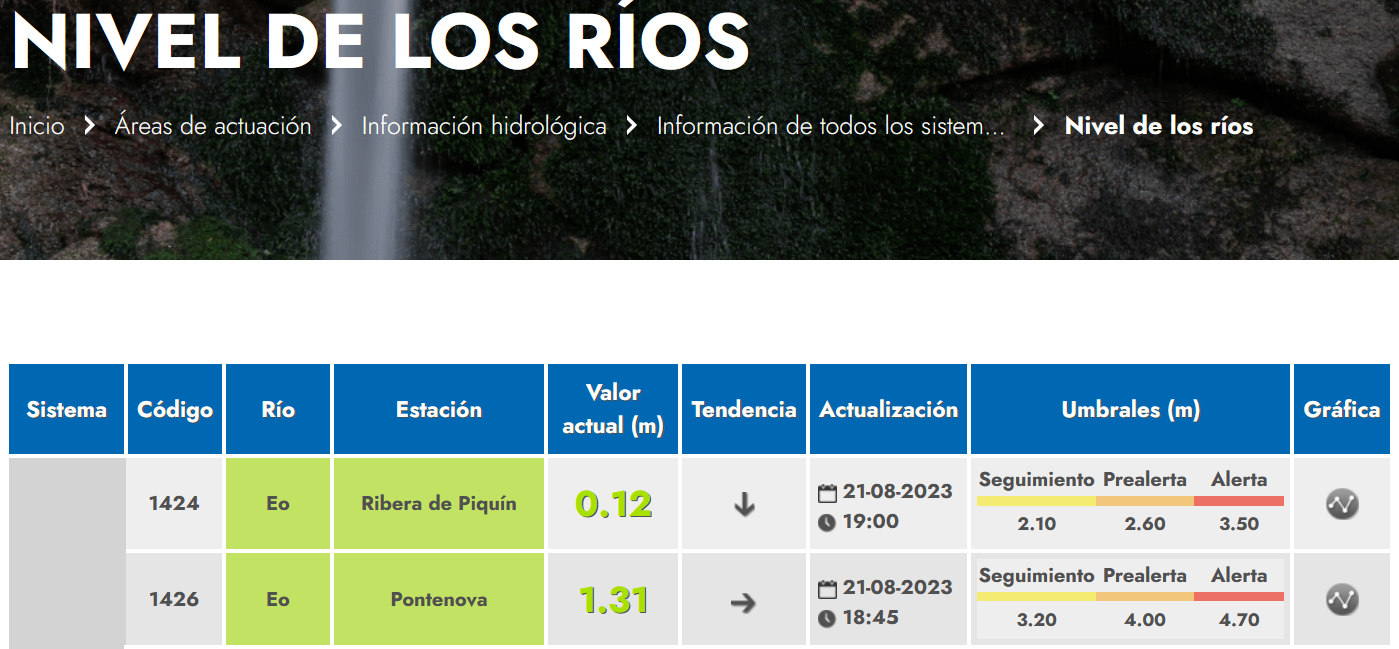
\includegraphics[width=.7\linewidth]{fig/CHCantabricoCode.png}
	\caption{Página Nivel de los ríos CHCantábrico}
	\label{fig:ej30}
\end{figure}

\begin{lstlisting}[basicstyle=\footnotesize, caption={HTML tabla estaciones en CHCantábrico}, label=cod:104]
	<table class="tablefixedheader niveles">
		<thead></thead>
		<tbody>
			<tr class="centrado">
				<td class="codigo">1207</td>
				<td class="verde">...</td>
				<td class="verde">...</td>
				<td class="valor">...</td>
				<td class="tendencia">...</td>
				<td class="actualizacion">...</td>
				<td>
					<table class="umbrales_gr">											
						<tbody></tbody>
					</table>
				</td>
				<td>...</td>	
			</tr>
			...
		</tbody>
	</table>
\end{lstlisting}

A diferencia del resto de las páginas visitadas, CHCantábrico no muestra los datos sobre la web, por el contrario, implementa un botón con el que descargarlos directamente en formato CSV. Los datos que se pueden obtener, son aquellos presentes en la tabla secundaria de las fila, los datos de pre-alerta, alerta y seguimiento para cada una de las estaciones, siendo datos valiosos a la hora de intentar anticipar inundaciones. Las coordenadas a su vez, tampoco vienen dados sobre la web, por lo que hace falta visitar la web del Centro de Estudios Hidrológicos (\url{https://ceh.cedex.es/}) para obtenerlas.

\section{Agencia estatal de Meteorología (Aemet)}
La figura \ref{fig:ej3} muestra la página web de Aemet, dentro podemos encontrar de forma accesible múltiples datos relacionados con la meteorología tomados cada hora, de los cuales seleccionaremos únicamente temperatura, precipitación y humedad, puesto que los datos relacionados con el viento no son tan relevantes para este proyecto. A su vez, no todas las estaciones muestran estos datos, ocurriendo lo mismo con los de presión atmosférica.

\begin{figure} [H]
	\centering
	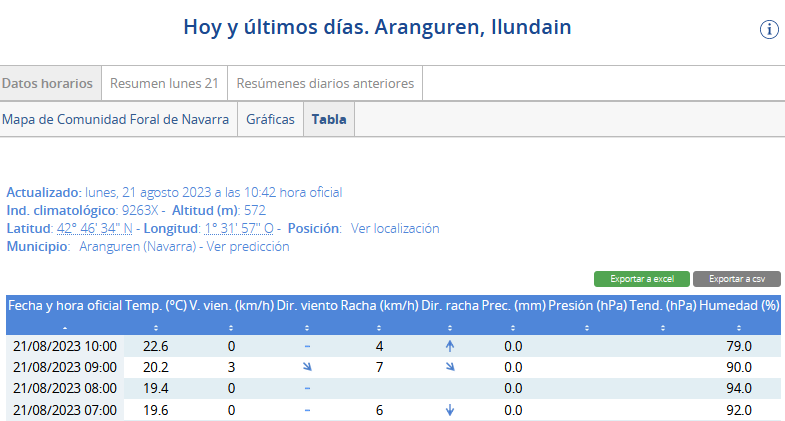
\includegraphics[width=0.7\textwidth]{fig/AemetData.png}
	\caption[Página Aemet de la estación en Aranguren (Navarra)]{Página Datos Aemet}
	\label{fig:ej3}
\end{figure}

\begin{lstlisting}[basicstyle=\footnotesize, caption={HTML tabla datos en Aemet}, label=cod:105]
	<table id="table">
		<thead></thead>
		<tbody>
			<tr class="fila_par">
				<td class="evenselected">27/08/2023 12:00</td>
				<td class="">16.6</td>
				<td class="">16</td>
				<td class="">...</td>
				<td class="">36</td>
				<td class="">...</td>
				<td class="">0.0</td>
				<td class=""> </td>
				<td class=""> </td>
				<td class="">67.0</td>
			</tr>
			...
		</tbody>
	</table>
\end{lstlisting}

Los datos en HTML vienen datos dentro de un elemento \textit{table}, lo que facilita su adquisición, pues permite tomar todas las filas (elementos \textit{tr}) pertenecientes al elemento \textit{tbody} de esta. Una vez obtenidas las filas, la forma de lograr los datos deseados seria eligir dentro de cada elemento \textit{tr} los elementos \textit{td} deseados, puesto que HTML empieza a contar elementos desde el uno (en vez de cero como suele ser común en lenguajes de programación), los \textit{td} a obtener serian: uno, fecha y hora; dos, temperatura; siete, precipitación; diez, humedad. como se aprecia en el código \ref{cod:105}

\begin{lstlisting}[basicstyle=\footnotesize, caption={HTML coordenadas en Aemet}, label=cod:106]
	<span class="geo">
		<span class="font_bold">Latitud</span>
		:
		<abbr class="latitude" title="42.7761111111">42 46' 34'' N</abbr>
		-
		<span class="font_bold">Longitud</span>
		:
		<abbr class="longitude" title="-1.5325000000">1 31' 57'' O</abbr>
		-
	</span>
\end{lstlisting}

Las coordenadas, dentro de un \textit{span}, están incluidas en elementos \textit{abbr} con sus respectivas clases \textit{''latitude``} y \textit{''longitude``}, haciendo posible su obtención fácilmente mediante los elementos \textit{abbr}. Presentes en código \ref{cod:106}.

\section{Meteorología y climatología de Navarra (MeteoNavarra)}
En la página de meteorología y climatología de Navarra encontramos una gran sección de estaciones de las cuales poder obtener datos, como se ve en la figura \ref{fig:ej27}.

\begin{figure} [H]
	\centering
	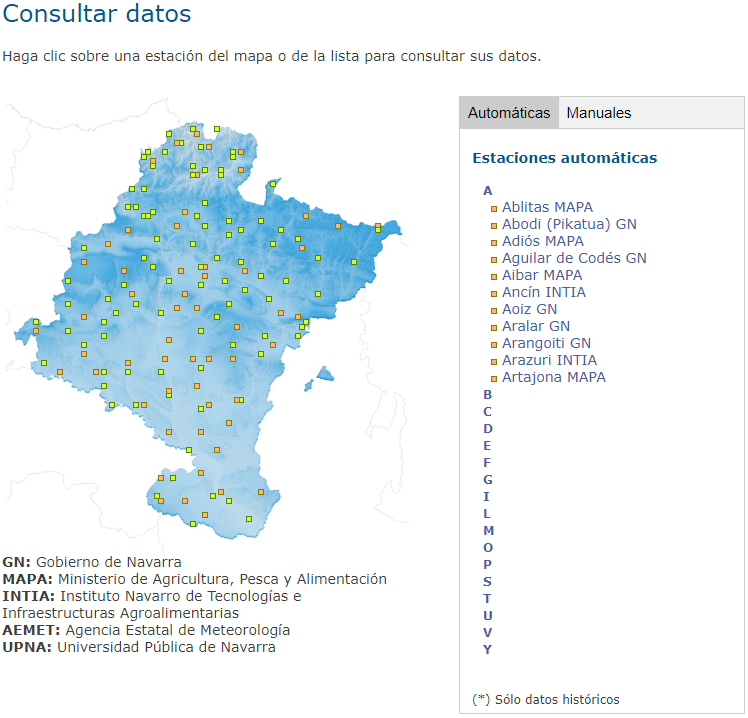
\includegraphics[width=0.7\textwidth]{fig/MeteoNavarraCode.png}
	\caption[Página estaciones MeteoNavarra]{Página estaciones MeteoNavarra}
	\label{fig:ej27}
\end{figure}

De entre los dos tipos e estaciones disponibles, automática y manual, únicamente se va a trabajar con los datos de las estaciones automáticas. El motivo de esto es que las manuales solo proveen datos diarios de, la temperatura máxima, mínima y de la precipitación acumulada. Esto hace que no se disponga de ningún dato hasta que finalice el día, cosa que no es viable si lo que se propone es predecir cambios radicales en un periodo de tiempo reducido.

\begin{lstlisting}[basicstyle=\footnotesize, caption={HTML tabla estaciones en MeteoNavarra}, label=cod:107]
	<table width="260" border="0" cellspacing="0">
		<tbody>
			<tr>
				<td colspan="2" height="470" valign="top">
					<div style="margin-left:5px; margin-right:5px;z-index:200">
						<div onclick="javascript:menu_openclose('AUTO_A');" style="width:100px;"></div>
						<div id="AUTO_A" style="margin-left:5px;display:none;">
							<script>
								doImage(274,6,'/img/2/estacionautomatica.gif','Ablitas MAPA','AUTO');
							</script>
							<img src="/img/spacer.gif" alt="" width="8" height="1" border="0">
							<img src="/img/2/estacionautomatica.gif" alt="Ablitas MAPA" width="6" height="6" border="0">
							<a href="estacion.cfm?IDestacion=274" onmouseover="showEstacion('274_info','6','AUTO')" onmouseout="hideEstacion('274_info','AUTO')"> Ablitas MAPA</a>
							<br>
							...
						</div>
						...
					</div>
					<br><br>
				</td>
			</tr>
		</tbody>
	</table>
\end{lstlisting}

Debido a la estructuración HTML usada para mostrar las estaciones vista en el código \ref{cod:107}, se puede ver que, aun usar el elemento \textit{table}, este solo dispone de una única fila y columna, haciendo de la columna un elemento \textit{div} sobre el que se insertan los datos.\newline
\newline
Las estaciones automáticas proporcionan tanto datos en periodos de diez minutos como datos diarios. Tras usar el mismo razonamiento que con las estaciones manuales, no tomamos los datos diarios y, entre los actualizados cada diez minutos, se toman la temperatura, humedad relativa, radiación global y precipitación. El resto se omitirán. como se muestra en la figura \ref{fig:ej6}.

\begin{figure} [H]
	\centering
	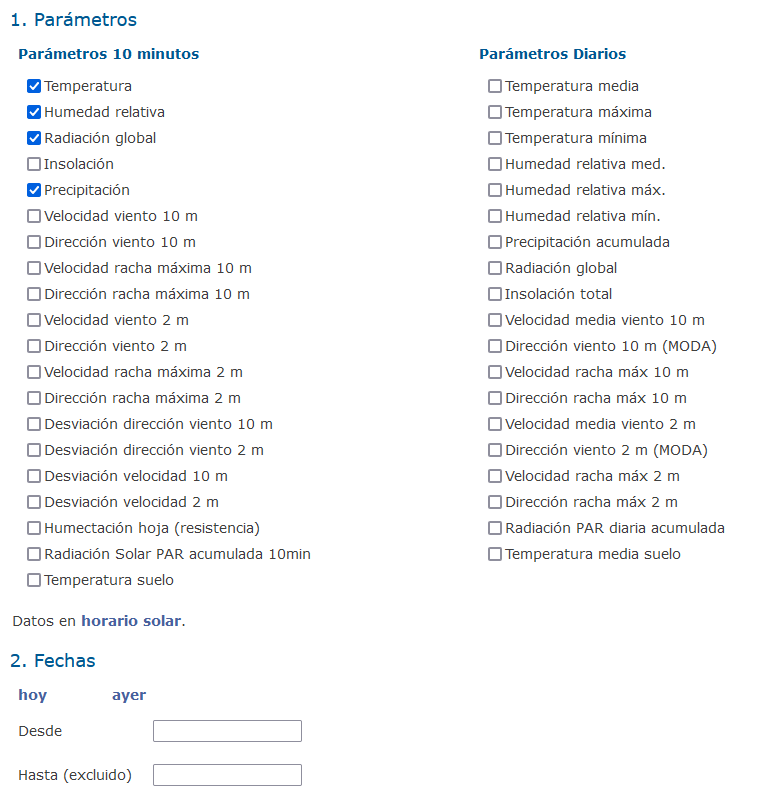
\includegraphics[width=0.6\textwidth]{fig/DatosMeteoNavarra.png}
	\caption[Apartado selección de datos MeteoNavarra]{Datos MeteoNavarra}
	\label{fig:ej6}
\end{figure}

Los datos se muestran en formato tabla, tanto visualmente, en la figura \ref{fig:ej29} como a nivel de HTML, en el código \ref{cod:108}, cosa que facilita su obtención.

\begin{figure} [H]
	\centering
	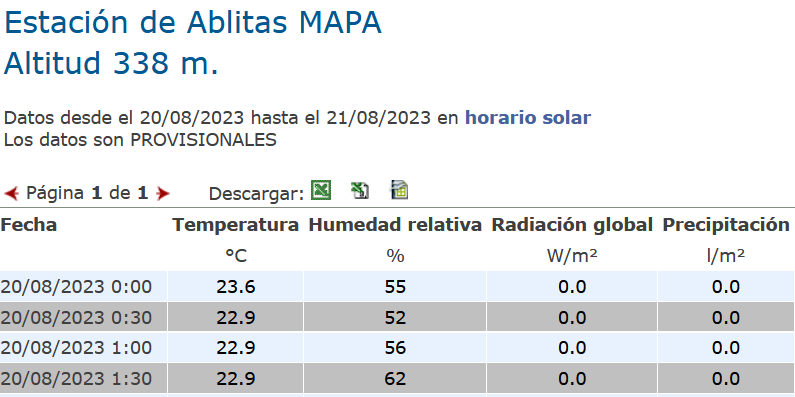
\includegraphics[width=.6\linewidth]{fig/MeteoNavarraData.png}
	\caption{Página de datos de MeteoNavarra}
	\label{fig:ej29}
\end{figure}

\begin{lstlisting}[basicstyle=\footnotesize, caption={HTML tabla datos en MeteoNavarra}, label=cod:108]
	<table class="border" border="0" cellpadding="3" cellspacing="1" bgcolor="#FFFFFF">
		<tbody>
			<tr bgcolor="#FFFFFF"></tr>
			<tr bgcolor="#FFFFFF"></tr>
			<tr bgcolor="E8F2FF">
				<td>26/08/2023 0:00</td>
				<td align="center">
					<font color="0">17.6</font>
				</td>
				<td align="center">
					<font color="0">82</font>
				</td>
				<td align="center">
					<font color="0">0.0</font>
				</td>
				<td align="center">
					<font color="0">0.0</font>
				</td>
			</tr>
			...
		</tbody>
	</table>
\end{lstlisting}

\section{El Agua en Navarra}
En esta página encontraremos los datos tanto del nivel de los ríos como de su caudal en los últimos 15 días en periodos de 10 minutos, siendo una de las fuentes principales de datos.
\newline
\newline
La sección de aforos en la página, mostrada en la figura \ref{fig:ej4}, muestra el mapa de Navarra junto a varias estaciones. Aunque no todas las disponibles en la web, conformando unicamente el grupo de estaciones principales.\newline
\newline
Con el fin de acceder a todas las estaciones disponibles, debemos centrarnos en el mapa de la esquina inferior derecha. Estructurada en 6 regiones, Norte, Arga, Ega, Ebro alto, Ebro bajo y Aragón, por medio de este mapa accedemos a cada región, mostrando el mapa de la región, dando acceso a todas las estaciones en la zona.

\begin{figure} [H]
	\centering
	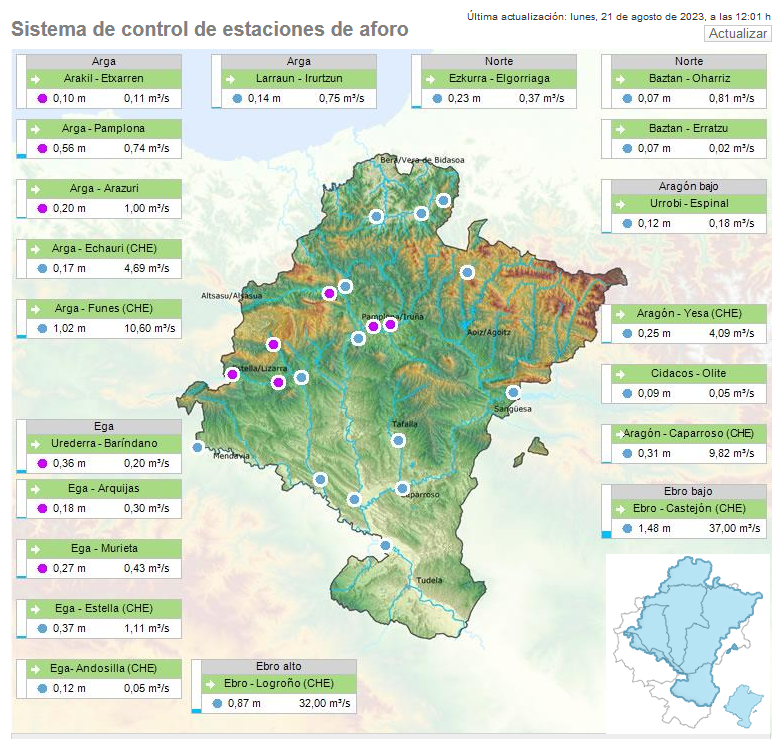
\includegraphics[width=0.7\textwidth]{fig/AguaEnNavarraCode.png}
	\caption[Página principal de aforos de El Agua en Navarra]{Página El Agua en Navarra}
	\label{fig:ej4}
\end{figure}

\begin{lstlisting}[basicstyle=\footnotesize, caption={HTML mapa estaciones en El Agua en Navarra}, label=cod:109]
	<map id="mapCajetines_mapa" name="mapCajetines">
		<area shape="rect" coords="5,5,180,59" alt="Arakil - Etxarren" href="https://administracionelectronica.navarra.es/aguaEnNavarra/ctaDatosEstacion.aspx?IdEstacion=50" onmouseover="javascript:document.getElementById('imgMapa').src='mostrarimagen.aspx?idMapa=1&"
		"amp;IdCajetin=62&amp;Vista=internet&amp;IdOrigenDatos=1'" target="_self" onmouseout="javascript:document.getElementById('imgMapa').src='mostrarimagen.aspx?idMapa=1&"
		"amp;Vista=internet&amp;IdOrigenDatos=1'">
		<area shape="circle" coords="317,243,11" alt="Arakil - Etxarren" href="https://administracionelectronica.navarra.es/aguaEnNavarra/ctaDatosEstacion.aspx?IdEstacion=50" onmouseover="javascript:document.getElementById('imgMapa').src='mostrarimagen.aspx?idMapa=1&"
		"amp;IdCajetin=62&amp;Vista=internet&amp;IdOrigenDatos=1'" target="_blank" onmouseout="javascript:document.getElementById('imgMapa').src='mostrarimagen.aspx?idMapa=1&"
		"amp;Vista=internet&amp;IdOrigenDatos=1'">
		...
	</map>
\end{lstlisting}

El HTML del mapa se estructura de la manera que se ve en el código \ref{cod:109}, mostrando un par de elementos \textit{area} por estación, uno con \textit{shape=''rect``}, representando las tarjetas que rodean el mapa y otro con \textit{shape=''circle``}, siendo los puntos en el mapa. Pulsar sobre cualquiera de ellos es equivalente, aunque posteriormente hagamos uso de los elementos con \textit{shape=''rect``} dentro del código.

\begin{figure} [H]
	\centering
	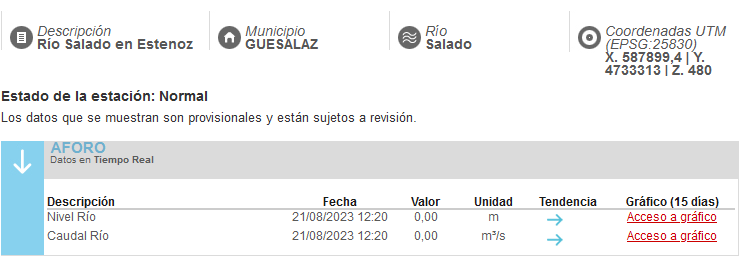
\includegraphics[width=0.7\textwidth]{fig/AguaEnNavarraEstacion.png}
	\caption[Página estación de El Agua en Navarra]{Página estación El Agua en Navarra}
	\label{fig:ej23}
\end{figure}

\begin{lstlisting}[basicstyle=\footnotesize, caption={HTML estaciones en El Agua en Navarra}, label=cod:110]
	<div id="bloq_iconos">
		<div id="descripcion">
			Descripcion
			<br>
			<span class="tit_icon">
				<span id="lblDescripcion">Urederra en Barindano</span>
			</span>
		</div>
		<div id="municipio">
			Municipio
			<br>
			<span class="tit_icon">
				<span id="lblMunicipio">Amescoa Baja</span>
			</span>
		</div>
		<div id="rio">
			Rio
			<br>
			<span class="tit_icon">
				<span id="lblRio">Urederra</span>
			</span>
		</div>
		<div id="coordenadas_UTM">
			Coordenadas UTM (EPSG:25830)
			<br>
			<span class="tit_icon">
				<span id="lblUTM">X. 571569,5 | Y. 4735145 | Z. 500</span>
			</span>
		</div>
	</div>
\end{lstlisting}

Las paginas de cada estación se muestran como en la figura \ref{fig:ej23}. De ella se obtienen los próximos datos, descripción, municipio, río y coordenadas. Ademas de dar acceso a los datos de nivel y caudal del río. Mostrados dentro de el \textit{div} con \textit{id=''blog\_icons``}. Una vez dentro del \textit{div} todos los datos siguen la misma estructuración, \textit{''//div/span/span``}, permitiendo la adquisición de todos los elementos a la vez. Como se aprecia en el codigo \ref{cod:110}\newline
\newline
Una vez se accede a los datos de la estación, se mostrara una gráfica como la de la figura \ref{fig:ej25}. A su vez, mediante el botón \textit{''Datos Numéricos``}, tendremos la posibilidad de observar los datos en forma numérica. Pero no sin antes haber visitado la versión gráfica. Pues da el error de la figura \ref{fig:ej5}.

\begin{figure} [H]
	\centering
	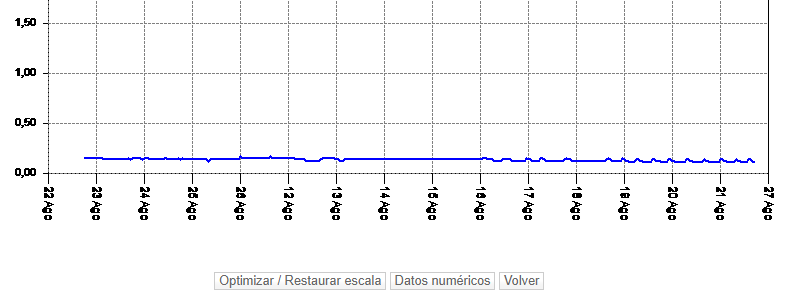
\includegraphics[width=0.7\textwidth]{fig/AguaEnNavarraGrafica.png}
	\caption[Gráfica de datos en estación de El Agua en Navarra]{Gráfica datos estación El Agua en Navarra}
	\label{fig:ej25}
\end{figure}

\begin{figure} [H]
	\centering
	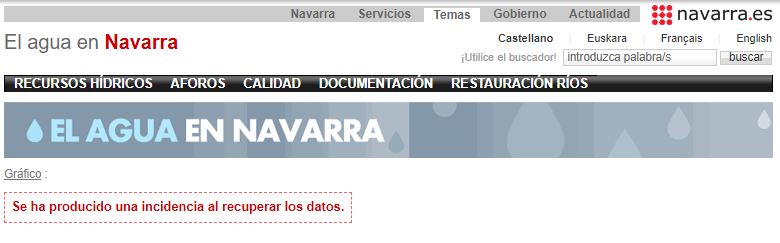
\includegraphics[width=0.7\textwidth]{fig/ErrorAguaEnNavarra.png}
	\caption[Error al cargar directamente la página de datos numéricos en El Agua en Navarra]{Error datos numéricos en El Agua en Navarra}
	\label{fig:ej5}
\end{figure}

Los datos numéricos están presentados en formato tabla como se aprecia en la figura \ref{fig:ej26}. Por el contrario, tras observar el HTML, en el código \ref{cod:111}, realmente es un elemento \textit{div}, que engloba los conjuntos de elementos \textit{span} que representan las lineas, separados por elementos \textit{br}. El formato en el que se presentan los datos, no hace más que representar una mayor complejidad para, posteriormente, trabajar y adquirir los datos. 

\begin{figure} [H]
	\centering
	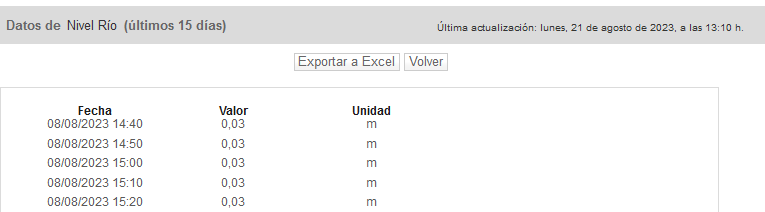
\includegraphics[width=.8\linewidth]{fig/AguaEnNavarraData.png}
	\caption{Datos numéricos de estaciones en Agua en Navarra}
	\label{fig:ej26}
\end{figure}

\begin{lstlisting}[basicstyle=\footnotesize, caption={HTML datos en El Agua en Navarra}, label=cod:111]
	<div id="lista">	                
		<span class="cont_fecha_gra">
			14/08/2023 16:10
		</span>
		<span class="cont_valor_gra">0,36</span>
		<span class="cont_unidad_gra">m</span>
		<span class="cont_vacio_gra"></span>
		<br>
		...
	</div>
\end{lstlisting}

De las webs mencionadas se dispone de los siguientes datos para este proyecto:

\begin{itemize}
	\setlength\itemsep{0.5em}
	\item Nivel (m)
	\item Caudal ($m^3/s$)
	\item Precipitación (mm)
	\item Temperatura (ºC)
	\item Humedad (\%)
	\item Radiación ($W/m^2$)
\end{itemize}

De Aemet: Temperatura, humedad y precipitación; en meteoNavarra: Temperatura, humedad, precipitación y radiación; aguaEnNavarra: Nivel y caudal del río; de CHCantábrico: Nivel del río, precipitación y seguimiento, alerta, pre-alerta del nivel. En todas las webs se proporciona las coordenadas junto con la fecha y hora en la que se ha hecho la medida.

A su vez, se dispone de la fecha y hora en la que se hizo la lectura de los datos, junto con los códigos y coordenadas de las estaciones sobre las cuales se obtienen los datos.